\section{Experiments}
\label{section 5}
In this section, we conduct experiments to demonstrate the effectiveness of RAHGNN for link prediction (LP) and node classification (NC) tasks.
\subsection{Experimental Setup}

\paragraph{Datasets.} 
We evaluate RAHGNN on five real world datasets including Cora~\cite{sen2008cora}, Citeseer~\cite{GCN}, Pubmed~\cite{namata2012PUBMED}, and the dataset statistics are shown in Table~\ref{banchmark dataset}. 
Since we focus on the hierarchy of the graph, we compute the Gromov’s $\delta$-hyperbolicity~\cite{jonckheere2008scaled,narayan2011large,adcock2013tree} for each graph dataset, where $\delta$ can measure how tree-like a graph is. 
A smaller $\delta$ means that the graph is more hyperbolicity, and while $\delta$ = 0 the graph is a tree. 

\begin{table}
\caption{Statistics of Datasets}
\centering
\begin{tabular}{lrrrrr}
\toprule
\textbf{Dataset} & \textbf{\# Nodes} & \textbf{\# Edges} & \textbf{\# Features} & \textbf{\# Classes} & $\delta$\\
\midrule
Cora     & 2,708  & 5,429  & 1,433 & 7   & 2.5 \\
Citeseer & 3,327  & 4,732  & 3,703 & 6   & 4 \\
Pubmed   & 19,717 & 44,327 & 500   & 3   & 2 \\
PPI      & 14,755  & 228,431 & 16    & 117 & 1 \\
WebKB    & 877    & 1,680   & 1,703  & 5   & 1 \\
\bottomrule
\end{tabular}
\label{banchmark dataset}
\end{table}

\begin{table*}[ht]
\caption{Summary of experimental results: “average accuracy±standard deviation”. }
\centering 
% \begin{adjustbox}{max width=0.95\linewidth}
\resizebox{\textwidth}{20mm}{
% \setlength{\tabcolsep}{2.5mm}{
\begin{tabular}{lccccccccccc}
\toprule
\textbf{Dataset} & \multicolumn{2}{c}{\textbf{Citeseer}} & \multicolumn{2}{c}{\textbf{Cora}} & \multicolumn{2}{c}{\textbf{Pubmed}} &
\multicolumn{2}{c}{\textbf{WebKB}} &
\multicolumn{2}{c}{\textbf{PPI}} &
\multirow{3}{*}{\textbf{Avg. Rank}}\\ 
\textbf{Hyperbolicity} $\delta$ & \multicolumn{2}{c}{$ \delta = 4 $} & \multicolumn{2}{c}{\textbf{$ \delta = 2.5 $}} & \multicolumn{2}{c}{\textbf{$ \delta = 2 $}} & \multicolumn{2}{c}{\textbf{$ \delta = 1 $}} &
\multicolumn{2}{c}{\textbf{$ \delta = 1 $}}\\ \cline{2-11}
\textbf{Task} & LP & NC & LP & NC & LP & NC & LP & NC & LP & NC\\
\midrule
MLP             & 76.39±0.02 &  74.70±0.01 &  57.45±0.01 &  59.50±0.01  &  68.27±0.02  &  72.40±0.00  & 72.33±0.00 & 72.22±0.01 & 51.62±0.01 & 37.10±0.02  & 7.5 \\
HNN~\cite{HNN:GaneaBH18}             & 87.81±0.01 &  79.20±0.04 &  84.65±0.02 &  60.04±0.01  &  82.04±0.00  &  72.90±0.01  & 79.38±0.01 & 81.82±0.01 & 51.13±0.00 & 36.47±0.02  & 6.3 \\
\midrule
GCN~\cite{GCN}             &         91.15±0.01  &       81.94±0.00 &          90.42±0.03  &         81.93±0.01  &        75.17±0.03  &         76.50±0.00  & 88.60±0.02 & 70.71±0.00 & 82.03±0.05 & 40.44±0.06 & 4.5 \\
GAT~\cite{GAT}             &         91.21±0.10  &         80.41±0.03  &   93.71±0.01 &         83.43±0.01  &         85.77±0.01 &         78.30±0.02 & 83.77±0.00 & 63.64±0.02 & 86.43±0.03 & 39.92±0.07  & 4.1 \\
GraphSTONE~\cite{topic2020}      &   86.08±0.06            &   54.56±0.03            &  \textbf{96.37±0.02} &  \textbf{84.73±0.02} & 94.25±0.01 &  78.61±0.02 & 78.07±0.01 & 51.74±0.01 & 78.24±0.01 & \textbf{43.64±0.02} & 4.3 \\
\midrule
GAT+HypeATT~\cite{HAtt}     &         91.33±0.05  &         81.27±0.01  &         90.68±0.01  &         80.26±0.01  &         91.30±0.01  &         75.32±0.01  & 87.49±0.01 & 82.16±0.03 & 86.17±0.04 & 40.02±0.03 & 4.0 \\
HGCN~\cite{HGCN_ChamiYRL19}            &         91.52±0.02  &         77.60±0.02  &         92.90±0.02 &         81.03±0.01  &         90.83±0.01  &         74.20±0.01  & 90.18±0.00 & 83.33±0.02 & 83.18±0.01 & 40.17±0.07 & 3.9 \\
\midrule
RAHGNN (Ours)    & \textbf{96.94±0.02} &  \textbf{85.28±0.01}  &       93.55±0.02  &  83.91±0.01 & \textbf{94.87±0.02} & \textbf{84.20±0.01}  & \textbf{94.32±0.00} & \textbf{83.38±0.00}   & \textbf{91.30±0.01} & 40.46±0.03 & \textbf{1.4} \\
\bottomrule
\end{tabular}}
% \end{adjustbox}
\label{summary results}
\end{table*}

\paragraph{Baselines.} 
We first compare RAHGNN with Neural Network models(MLP, HNN~\cite{HNN:GaneaBH18}) in Euclidean space and hyperbolic space, respectively. 
Then we compare our method to two classic Euclidean GNNs based methods (GCN~\cite{GCN} and GAT~\cite{GAT}) and an improved GNNs with advanced topology and node feature fusion capability (GraphSTONE~\cite{topic2020}). 
We also compare with two hyperbolic methods (H-GAT~\cite{HAtt} and HGCN~\cite{HGCN_ChamiYRL19}). 
%AM-GCN~\cite{am-gcn2020} and%
To put it in another way, excessive use of topology information inhibits the capability of learning node features. 

\begin{figure}[htpb]
	\centering
	\subfigure[Training loss of LP on Citeseer.]{
		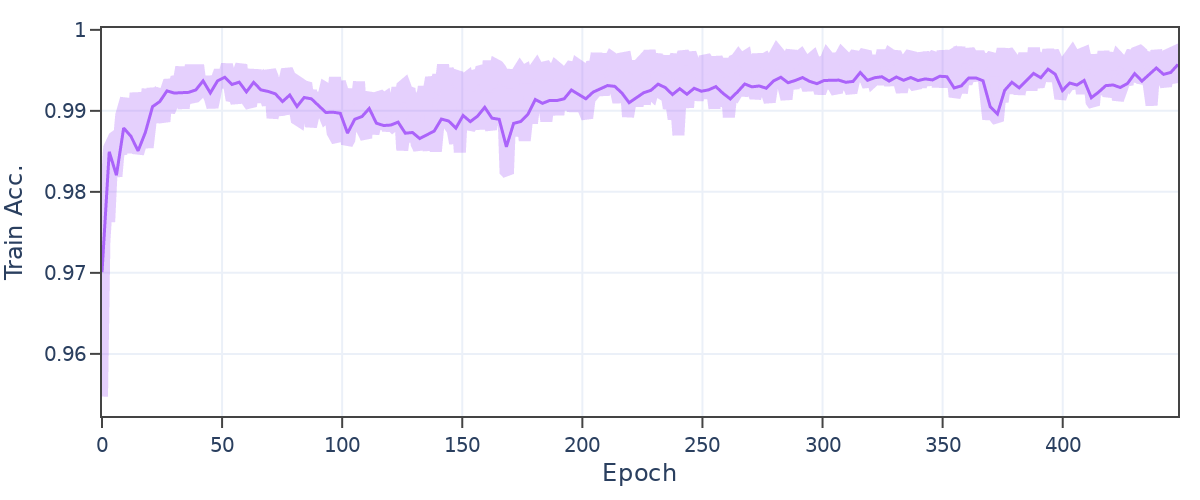
\includegraphics[width=0.22\textwidth]{figure/loss_citeseer_lp.png}
	}
	\subfigure[Training loss of NC on Citeseer.]{
		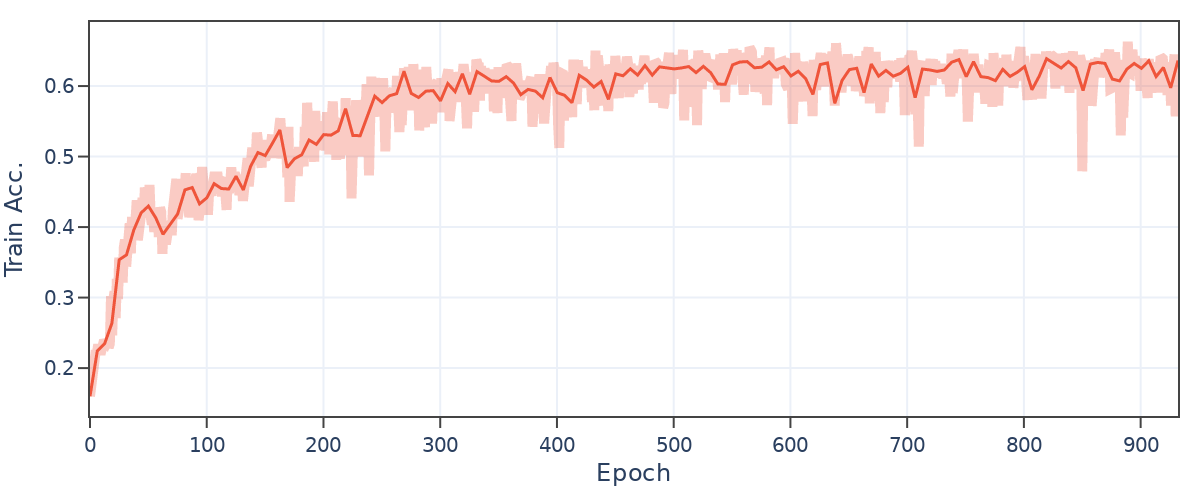
\includegraphics[width=0.22\textwidth]{figure/loss_citeseer_nc.png}
	}\\
	\subfigure[Training loss of LP on Cora.]{
		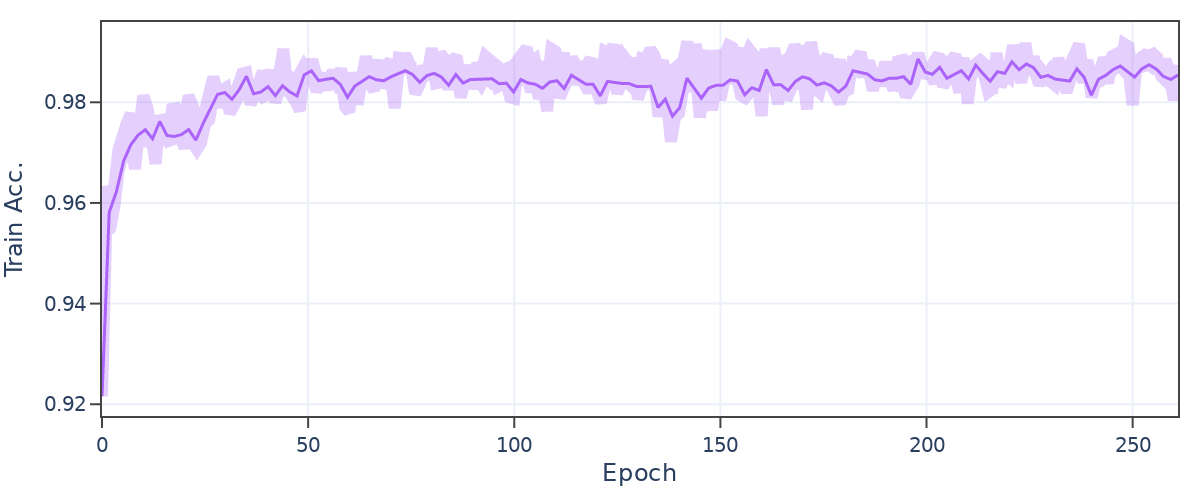
\includegraphics[width=0.22\textwidth]{figure/loss_cora_lp.png}
	}
	\subfigure[Training loss of NC on Cora.]{
		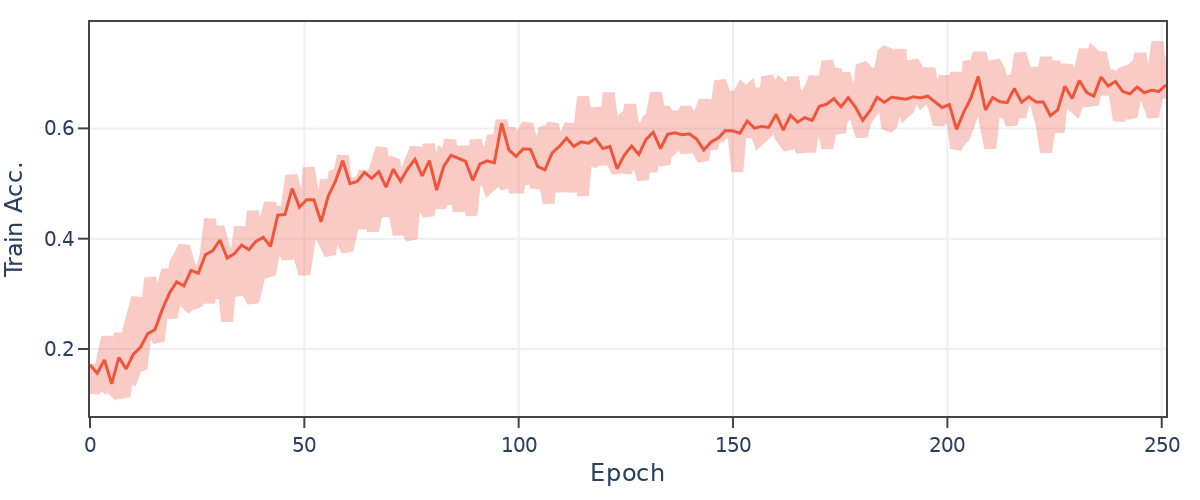
\includegraphics[width=0.22\textwidth]{figure/loss_cora_nc.png}
	}\\
	\subfigure[Training loss of LP on WebKB.]{
		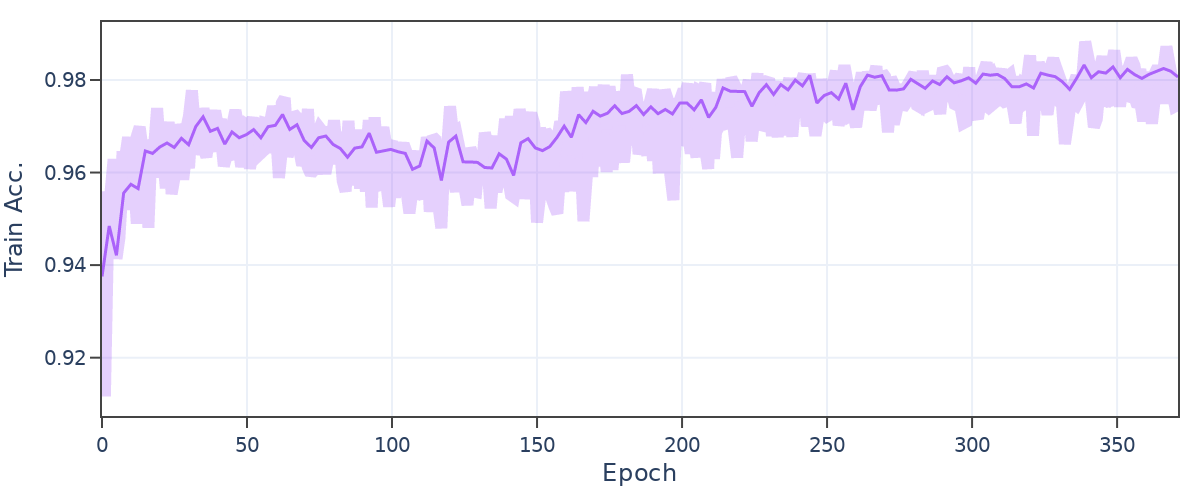
\includegraphics[width=0.22\textwidth]{figure/loss_webkb_lp.png}
	}
	\subfigure[Training loss of NC on WebKB.]{
		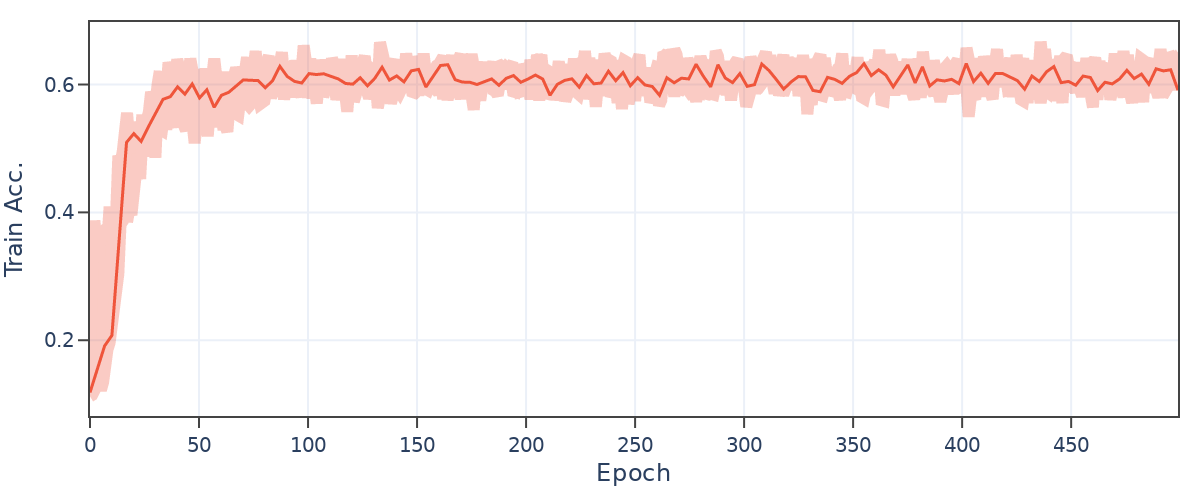
\includegraphics[width=0.22\textwidth]{figure/loss_webkb_nc.png}
	}
    % \vspace{-5pt}
	\caption{RL process analysis of RAHGNN.}
% 	\vspace{-10pt}
	\label{LP-C}
\end{figure}
\vspace{-0.6em}

\paragraph{Settings.}
We unify the output embedding with 16-dimensional vectors, and adopt Riemannian Adam optimizer~\cite{NickelK17Poincare} with a learning rate from 1e-4 to 5e-4, a weight-decay value of 5e-3, and a dropout value of 0.5. 
For GNNs (GCN, GAT and GraphSTONE), we set a 2-layer network while the dimension of the hidden layer is also 16. 
For unique parameters in GraphSTONE and HGCN, we adopt their default value setting as same as their paper. 
For our own model, we set the initial curvature $K=-1$ for multi-agent reinforcement learning. 
We run 5 times with the same parameter settings and report the average results. 
We utilize the ROC-AUC as the metric of link prediction, and F1 score as the metric of node classification. 

We also evaluate our method in two learning settings (i.e., transductive and inductive) for the node classification task. 
(1) \textit{Transductive}. 
We allow all models access to the whole graph (i.e., all edges and node features). 
We apply this setting for Cora, Pubmed, Citeseer, WebKB. 
(2) \textit{Inductive}. 
The test nodes are unobserved during training. We apply this setting on PPI, where we train all GNNs on 20 graphs and directly predict on two fixed test graphs as in~\cite{hamilton2017inductive}. 

\begin{figure}[htp]
	\centering
	\subfigure[LP on Citeseer.]{
		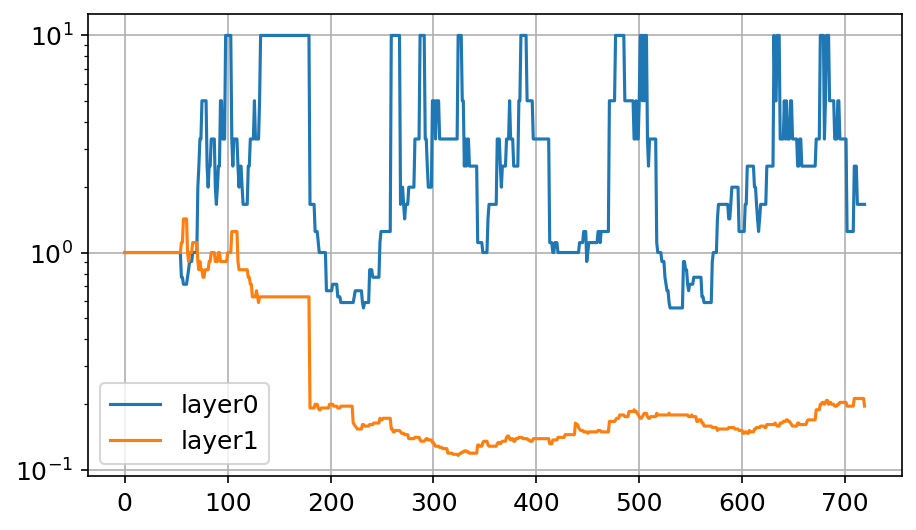
\includegraphics[width=0.18\textwidth]{figure/lp-citeseer-agent1_.png}
	}
	\hspace{5pt}
	\subfigure[NC on Citeseer.]{
		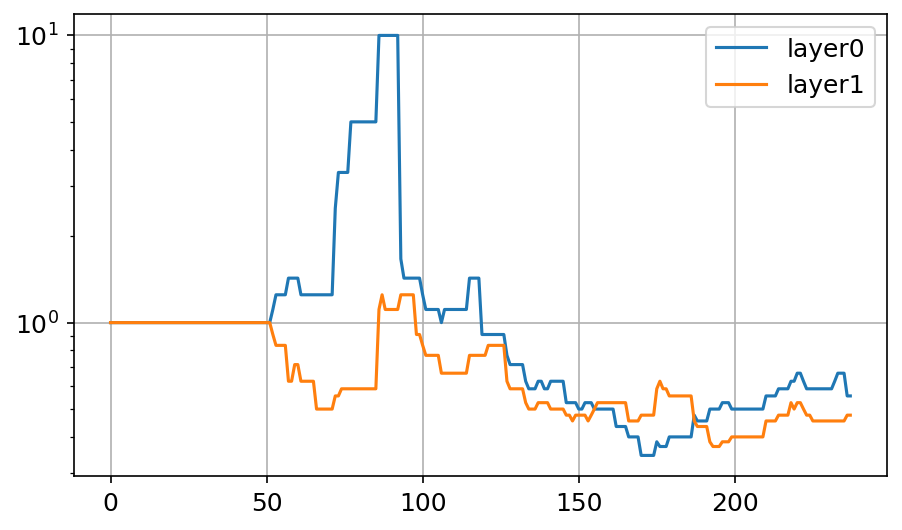
\includegraphics[width=0.18\textwidth]{figure/nc-citeseer-agent1_take.png}
	}\\
	\vspace{-10pt}
	\subfigure[LP on Cora.]{
		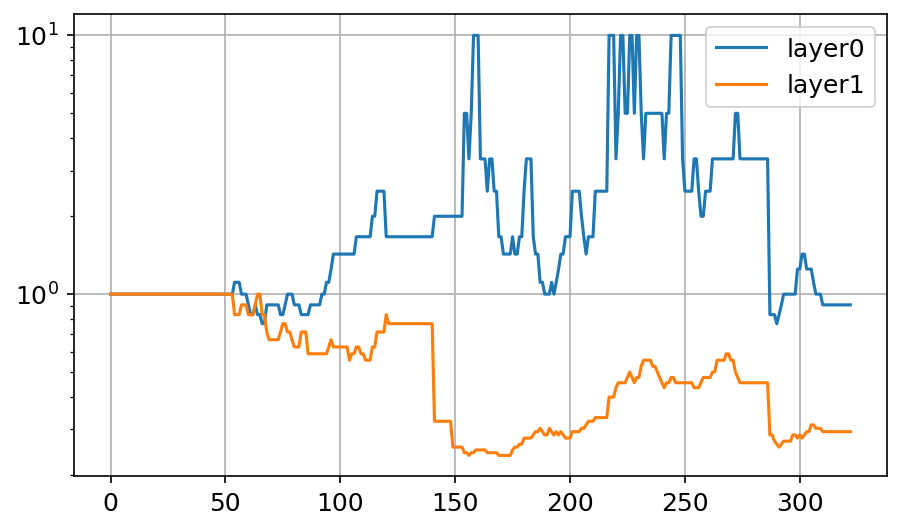
\includegraphics[width=0.18\textwidth]{figure/lp-cora-agent1_take.png}
	}
	\hspace{5pt}
	\subfigure[NC on Cora.]{
		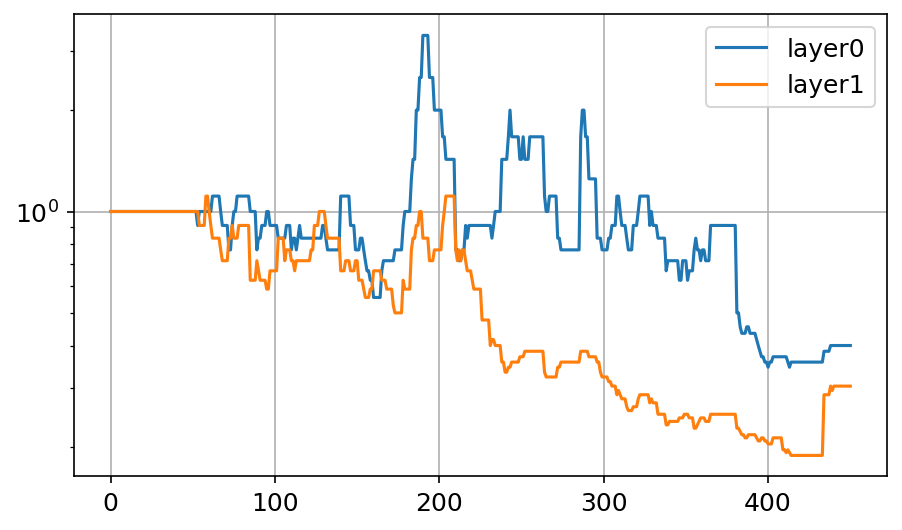
\includegraphics[width=0.18\textwidth]{figure/nc-cora-agent1_take.png}
	}\\
	\vspace{-10pt}
	\subfigure[LP on WebKB.]{
		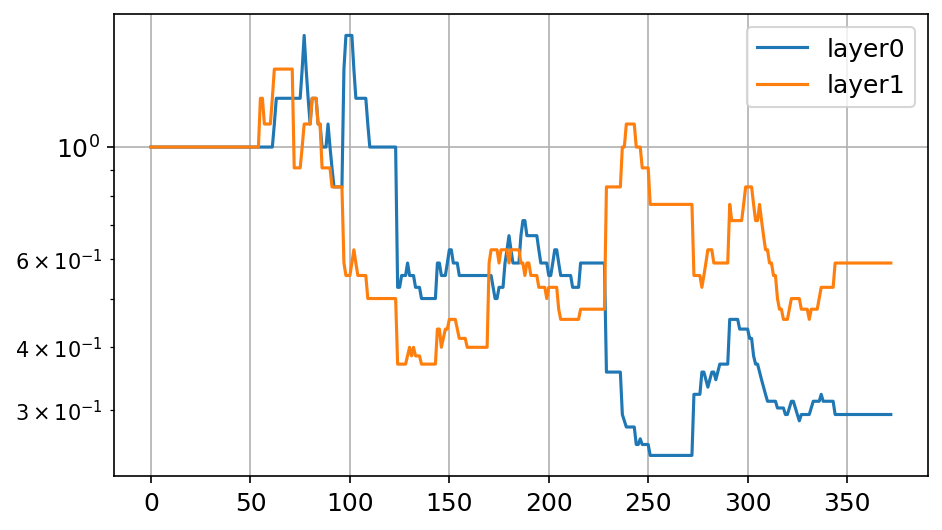
\includegraphics[width=0.18\textwidth]{figure/lp-webkb-agent1.png}
	}
	\hspace{5pt}
	\subfigure[NC on WebKB.]{
		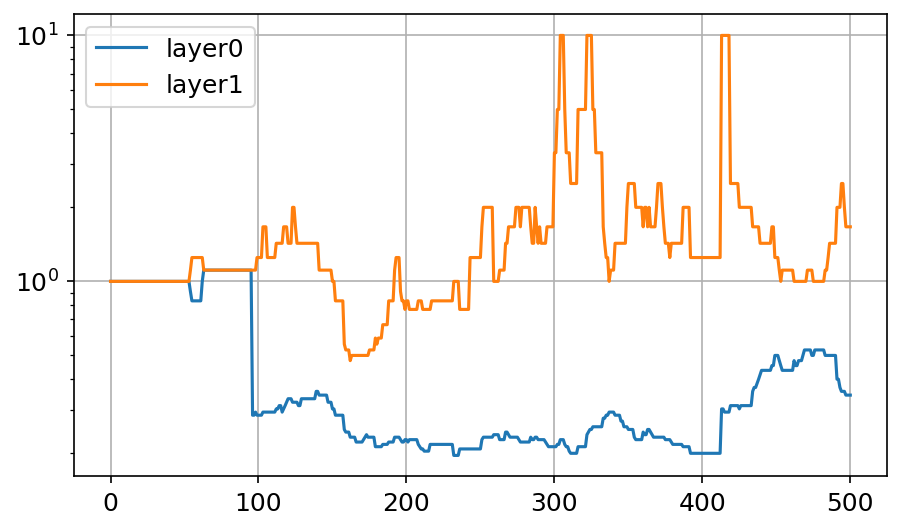
\includegraphics[width=0.18\textwidth]{figure/nc-webkb-agent1_.png}
	}
	\vspace{-1pt}
	\caption{Curvature updating process of RAHGNN.}
% 	\vspace{-0.6em}
	\label{RL_loss}
\end{figure}
\vspace{-0.6em}


\subsection{Quantitative Evaluation}
% \paragraph{Performance} 
We conduct experiments on link prediction and node classification to quantitatively evaluate our proposed model. 
Table~\ref{summary results} reports the performance of RAHGNN and baseline methods. 
We can get the observation: 
(1) Hyperbolic GNNs (HGNN, HGCN and our RAHGNN) perform better in the higher hyperbolicity (lower $\delta$) datasets where both node features and hierarchical topology play an important role. 
(2) For lower hyperbolicity (higher $\delta$) data sets, our model performs better than other hyerpbolic GNNs (HGNN and HGCN). 
Moreover, For the Euclidean GNNs method, our performance was close to theirs, and our model was even better on Citeseer.

In conclusion, the extensive experiments demonstrate the adaptability of our model on datasets with different hyperbolicity.Although the results on some datasets with lower curvature are close to or even slightly lower than the results of models in Euclidean space, our model generally performs better on datasets with higher curvature (such as pubmed, webkb). The overall rank also proves that the adaptability of RAHGNN exceeds traditional model.

\subsubsection{Link Prediction}
% Link prediction aims to predict whether there is an edge between two un-trained nodes according to the training result. 
% We conduct link prediction using all datasets, comparing effect with all baselines.
% We sample certain proportion of nodes and links from the network, marking them with positive tags and negative tags, and compute cross entropy as the loss function. 
We conduct link prediction using all datasets, comparing the performance with all baselines.
We sample a proportion of nodes and edges from the network, marking them with identical number of positive tags and negative tags.

% The results are shown in Table~\ref{summary results}. 
% With the collaborative reinforcement learning algorithm, our model could adjust curvatures more flexibly and explore better curvature values, enhancing the ability of link prediction. 
% As shown in Table~\ref{summary results}, our model conspicuously outperforms the conventional method, demonstrating the advantages of Hyperbolic Manifold instead of Euclidean Manifold. 
The results are shown in Table~\ref{summary results}. 
With the collaborative reinforcement learning algorithm, our model can obtain more accurate embeddings of initial networks by flexibly adjusting curvatures and exploring better curvature values.
RAHGNN conspicuously outperforms the conventional method, demonstrating that GNNs can markedly benefit from hyperbolic geometry.
\subsubsection{Node Classification}
We evaluate our model and all baselines in the node classification task. 
Since PPI contains disjoint graphs, we merge the adjacent matrices of all graphs into one big adjacent matrix. 
Then we use the nodes of 20 graphs as training samples and the others as test samples. 
In this way, all datasets could fit in transductive settings so that the evaluation criteria could be unified. 

\noindent \textbf{Transductive classification.} 
The results of transductive node classification in Cora and Pubmed are shown in Table 2. RAHGNN performs well in transductive datasets, and the overall rank is much higher than conventional baselines.    

\noindent \textbf{Inductive classification.} 
The results of inductive node classification in PPI are shown in Table 2.
RAHGNN also outperforms conventional models like GNNs, indicating that our model well captures the node features of graphs. 

\begin{figure*}[ht]
\centering
\subfigure[GCN]{
\includegraphics[width=0.20\linewidth]{figure/GCN_cora_visualization.png}
%\caption{fig1}
}%
\hspace{15pt}
\subfigure[GAT]{
\includegraphics[width=0.20\linewidth]{figure/GAT_cora_visualization.png}
%\caption{fig2}
}%
\hspace{15pt}
\subfigure[HGCN ($K=-0.832$)]{
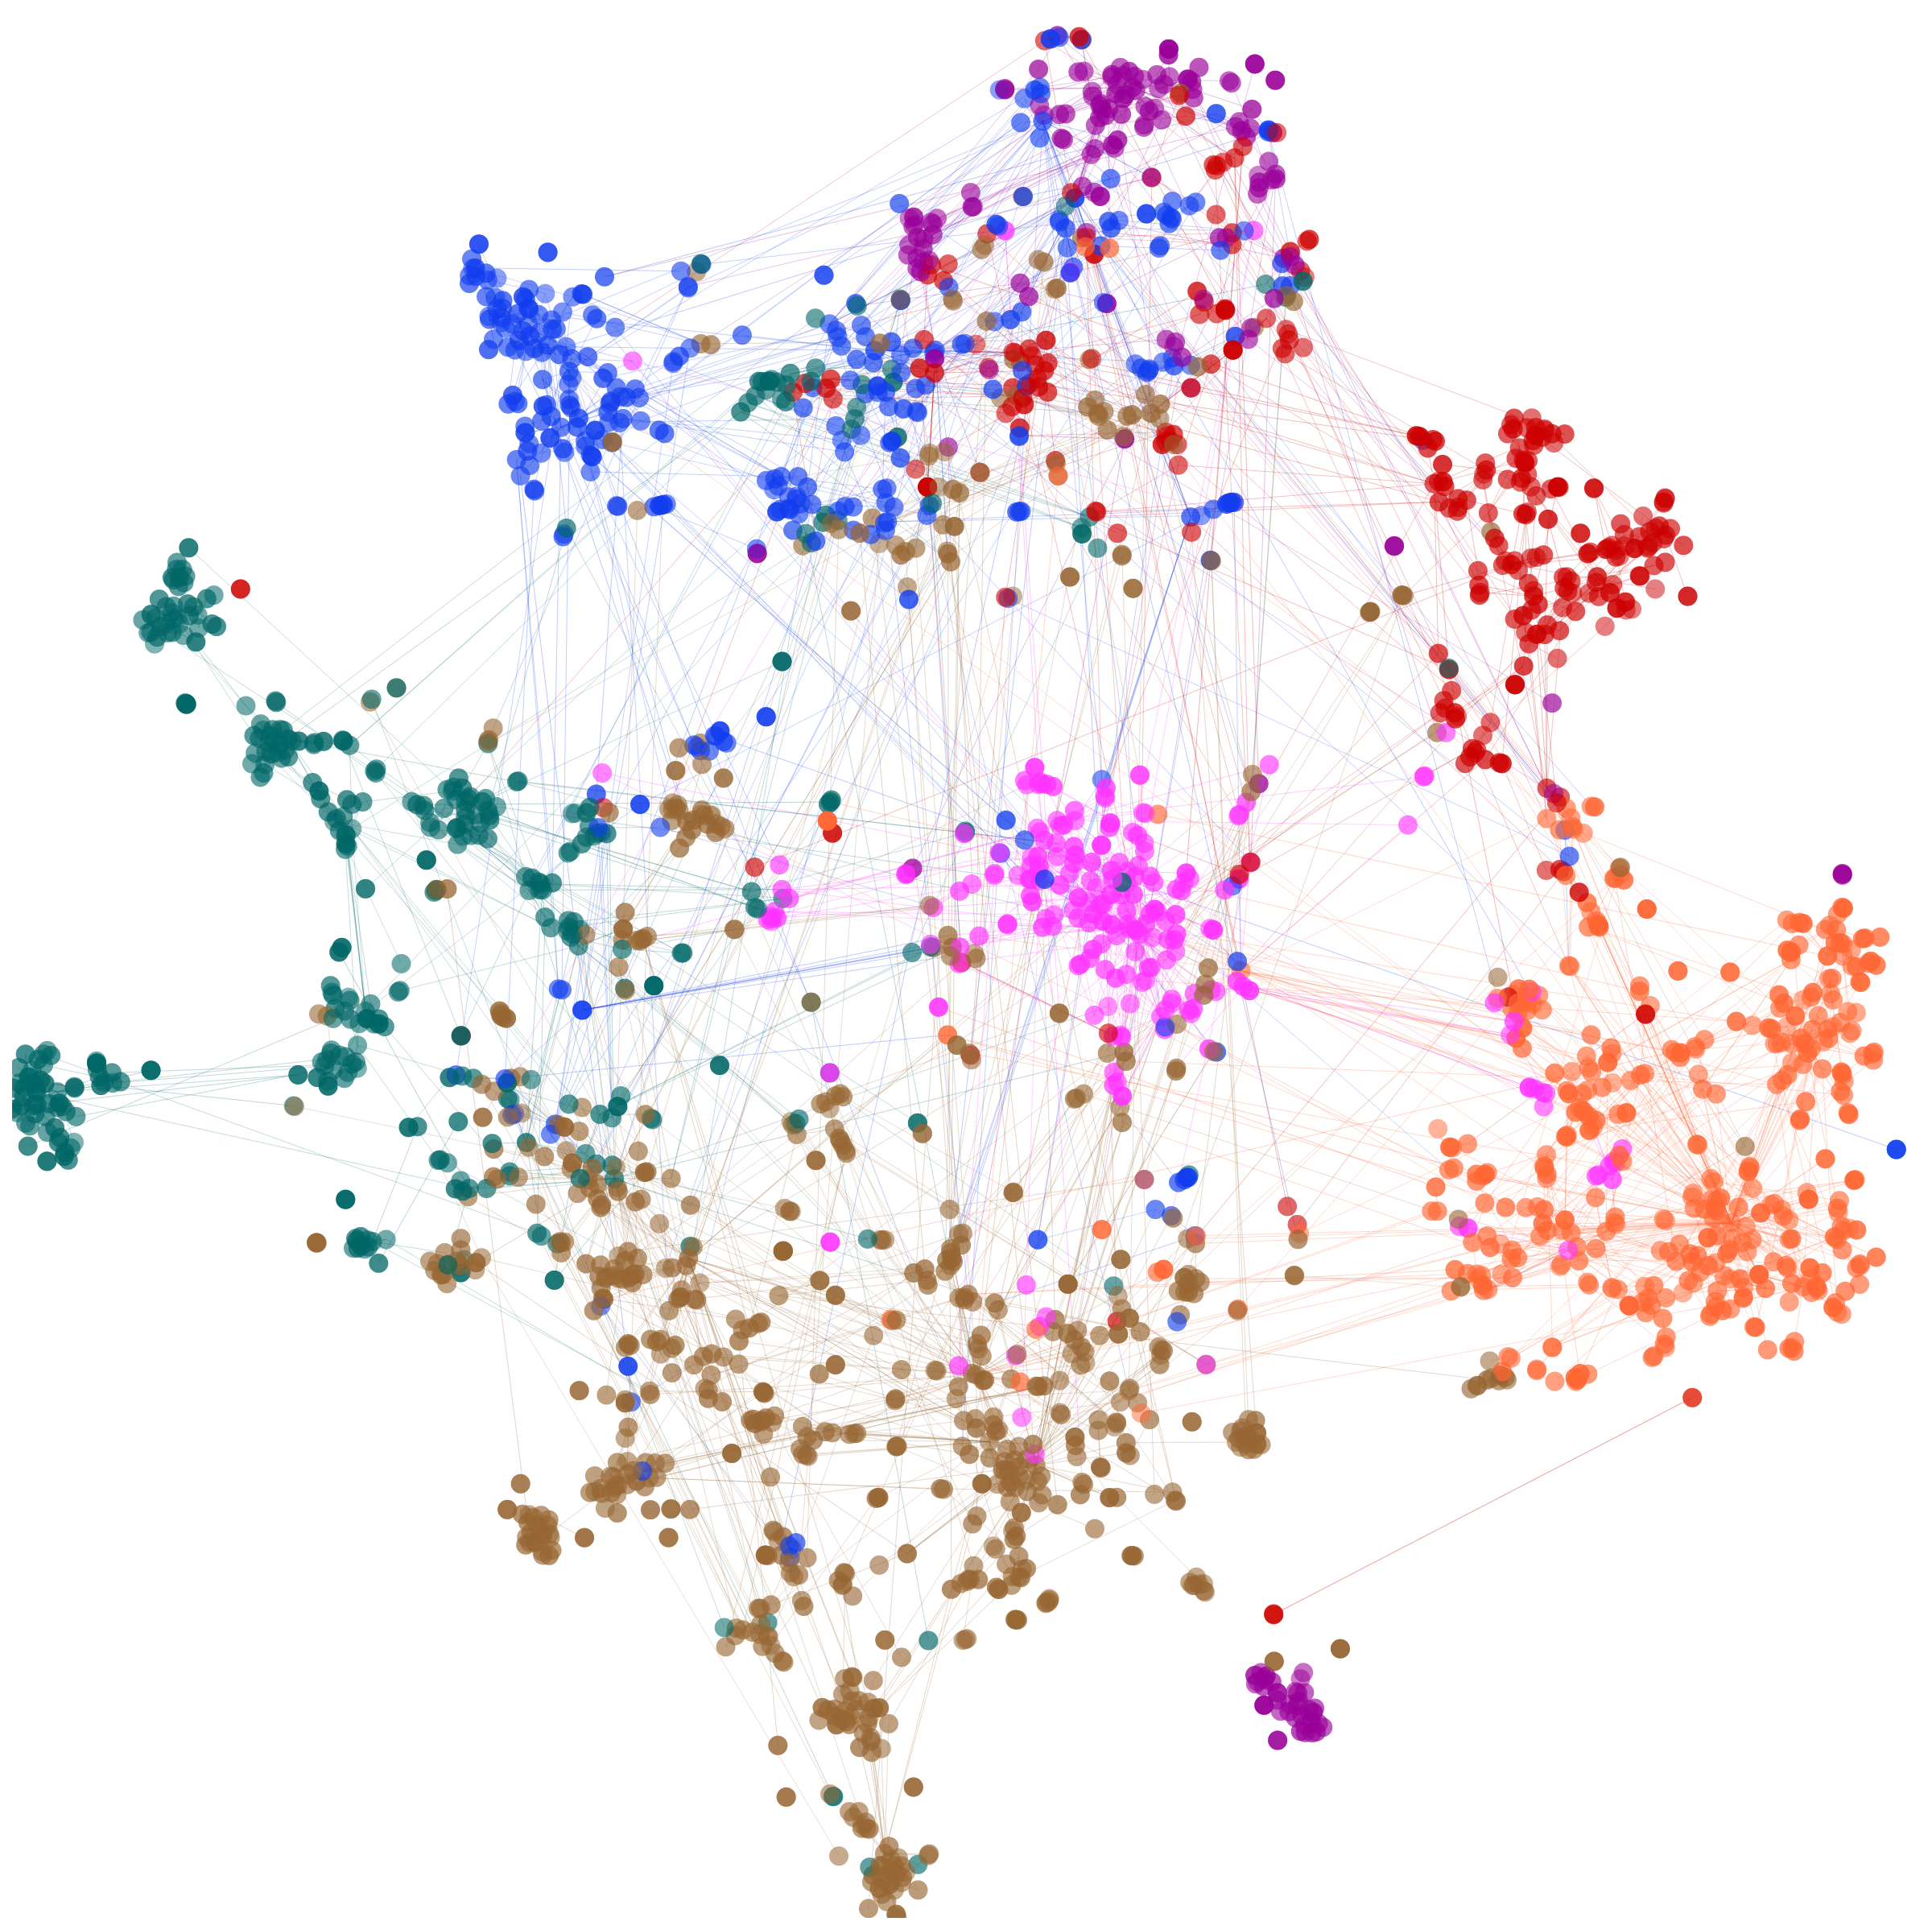
\includegraphics[width=0.20\linewidth]{figure/HGCN_cora_visualization.png}
}
\hspace{15pt}
\subfigure[RAHGNN ($K=-0.436$)]{
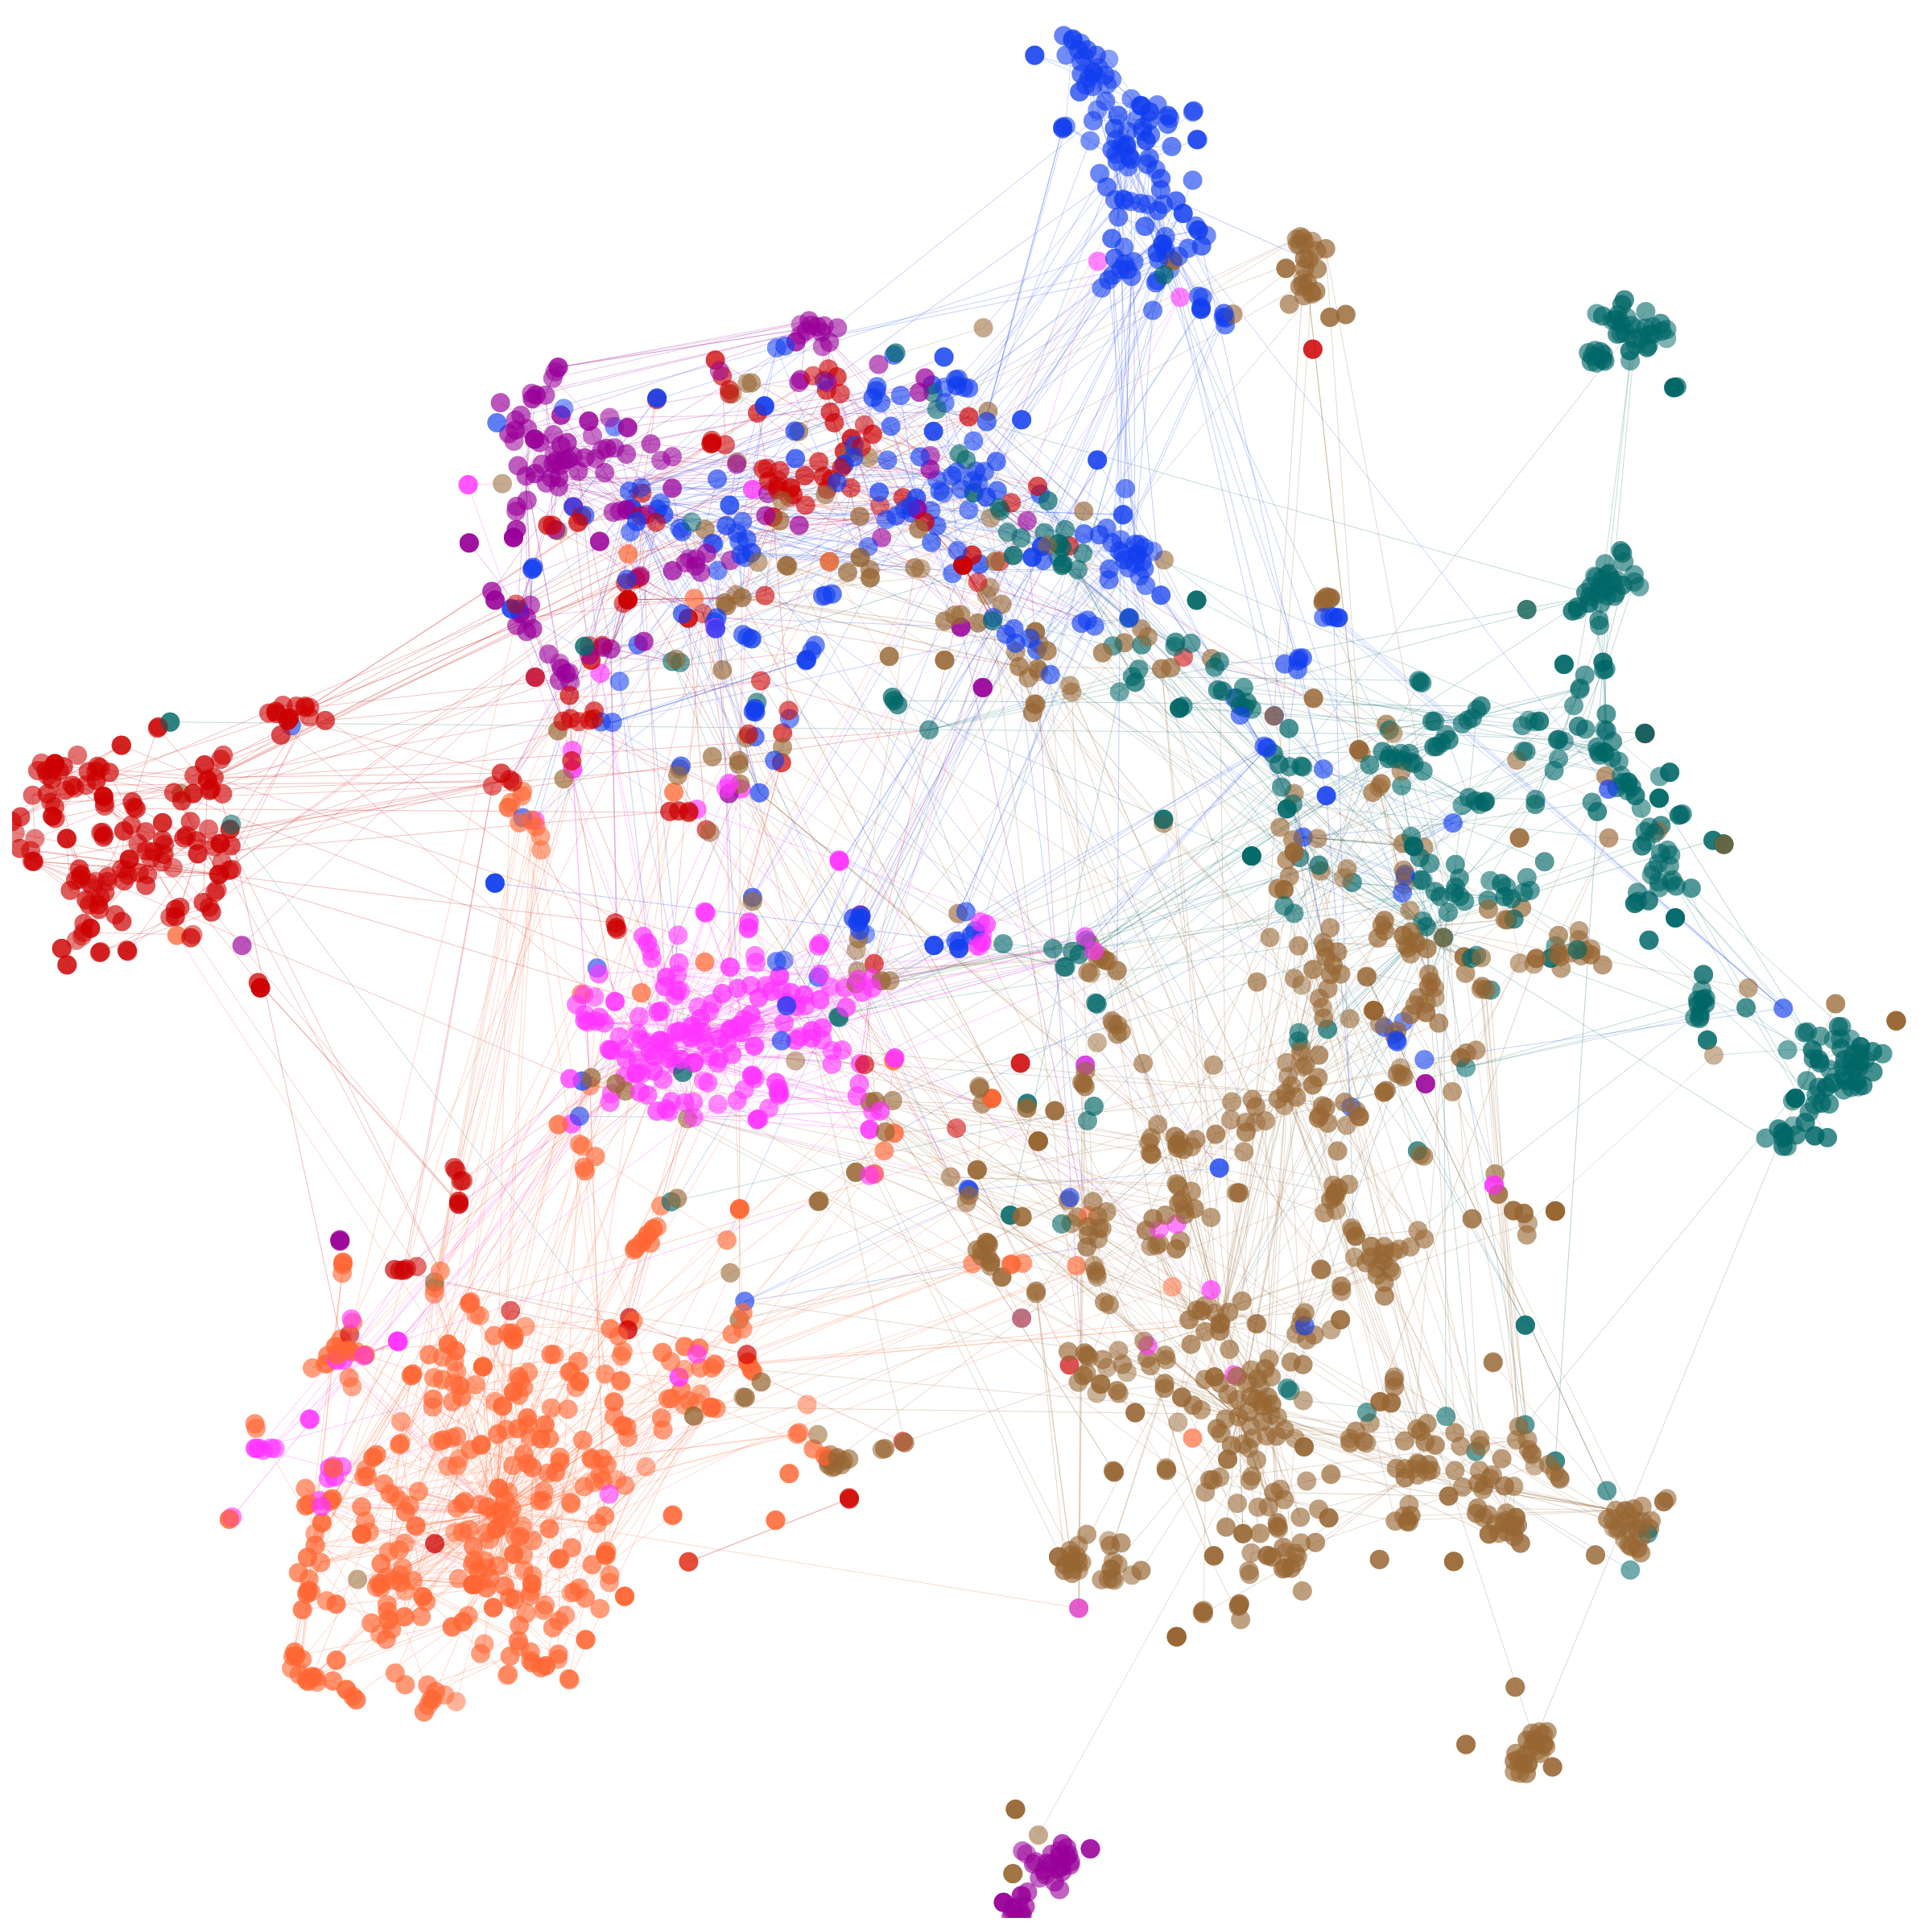
\includegraphics[width=0.20\linewidth]{figure/RHGNN_cora_visualization.png}
}
\centering
\caption{Visualization of node embeddings of different models on Cora.}
\label{visualization1}
\end{figure*}

\begin{figure*}[ht]
\centering
\subfigure[Citeseer $\delta = 4$]{
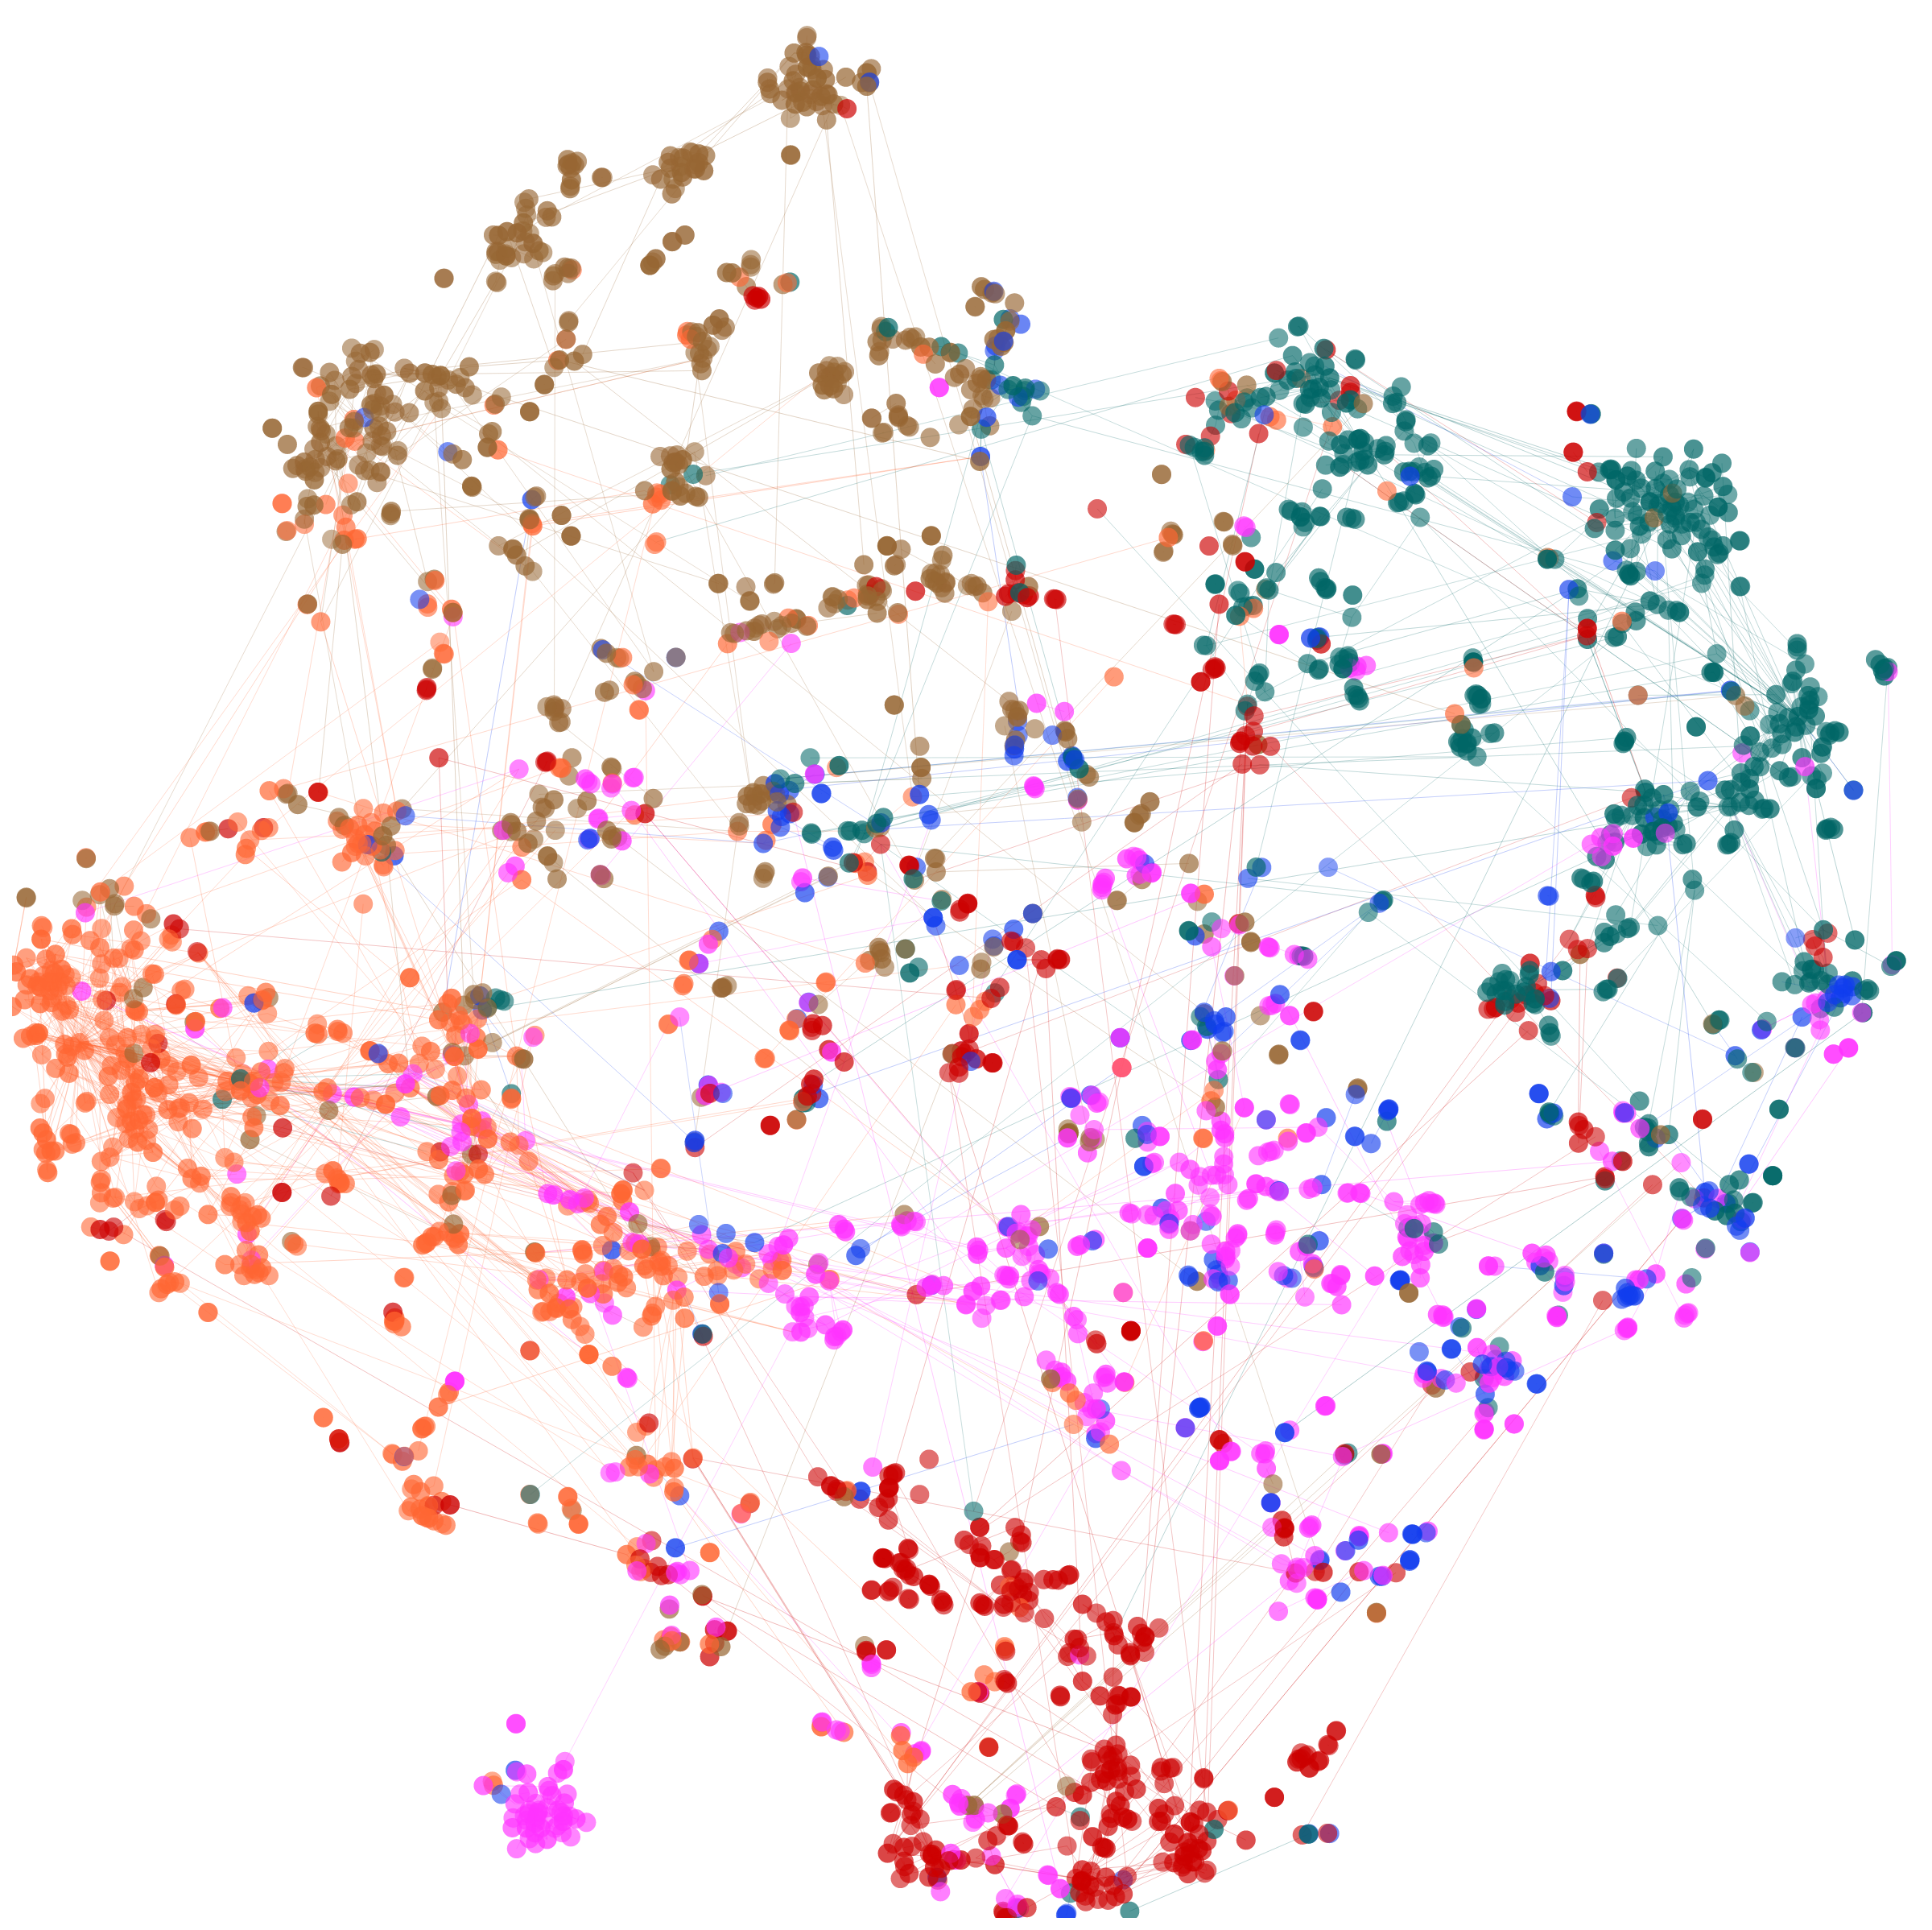
\includegraphics[width=0.15\linewidth]{figure/RHGNN_citeseer_visualization.png}
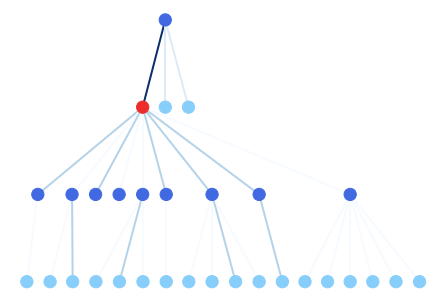
\includegraphics[width=0.15\linewidth]{figure/citeseer_att.png}
}
\subfigure[Cora $\delta = 2.5$]{
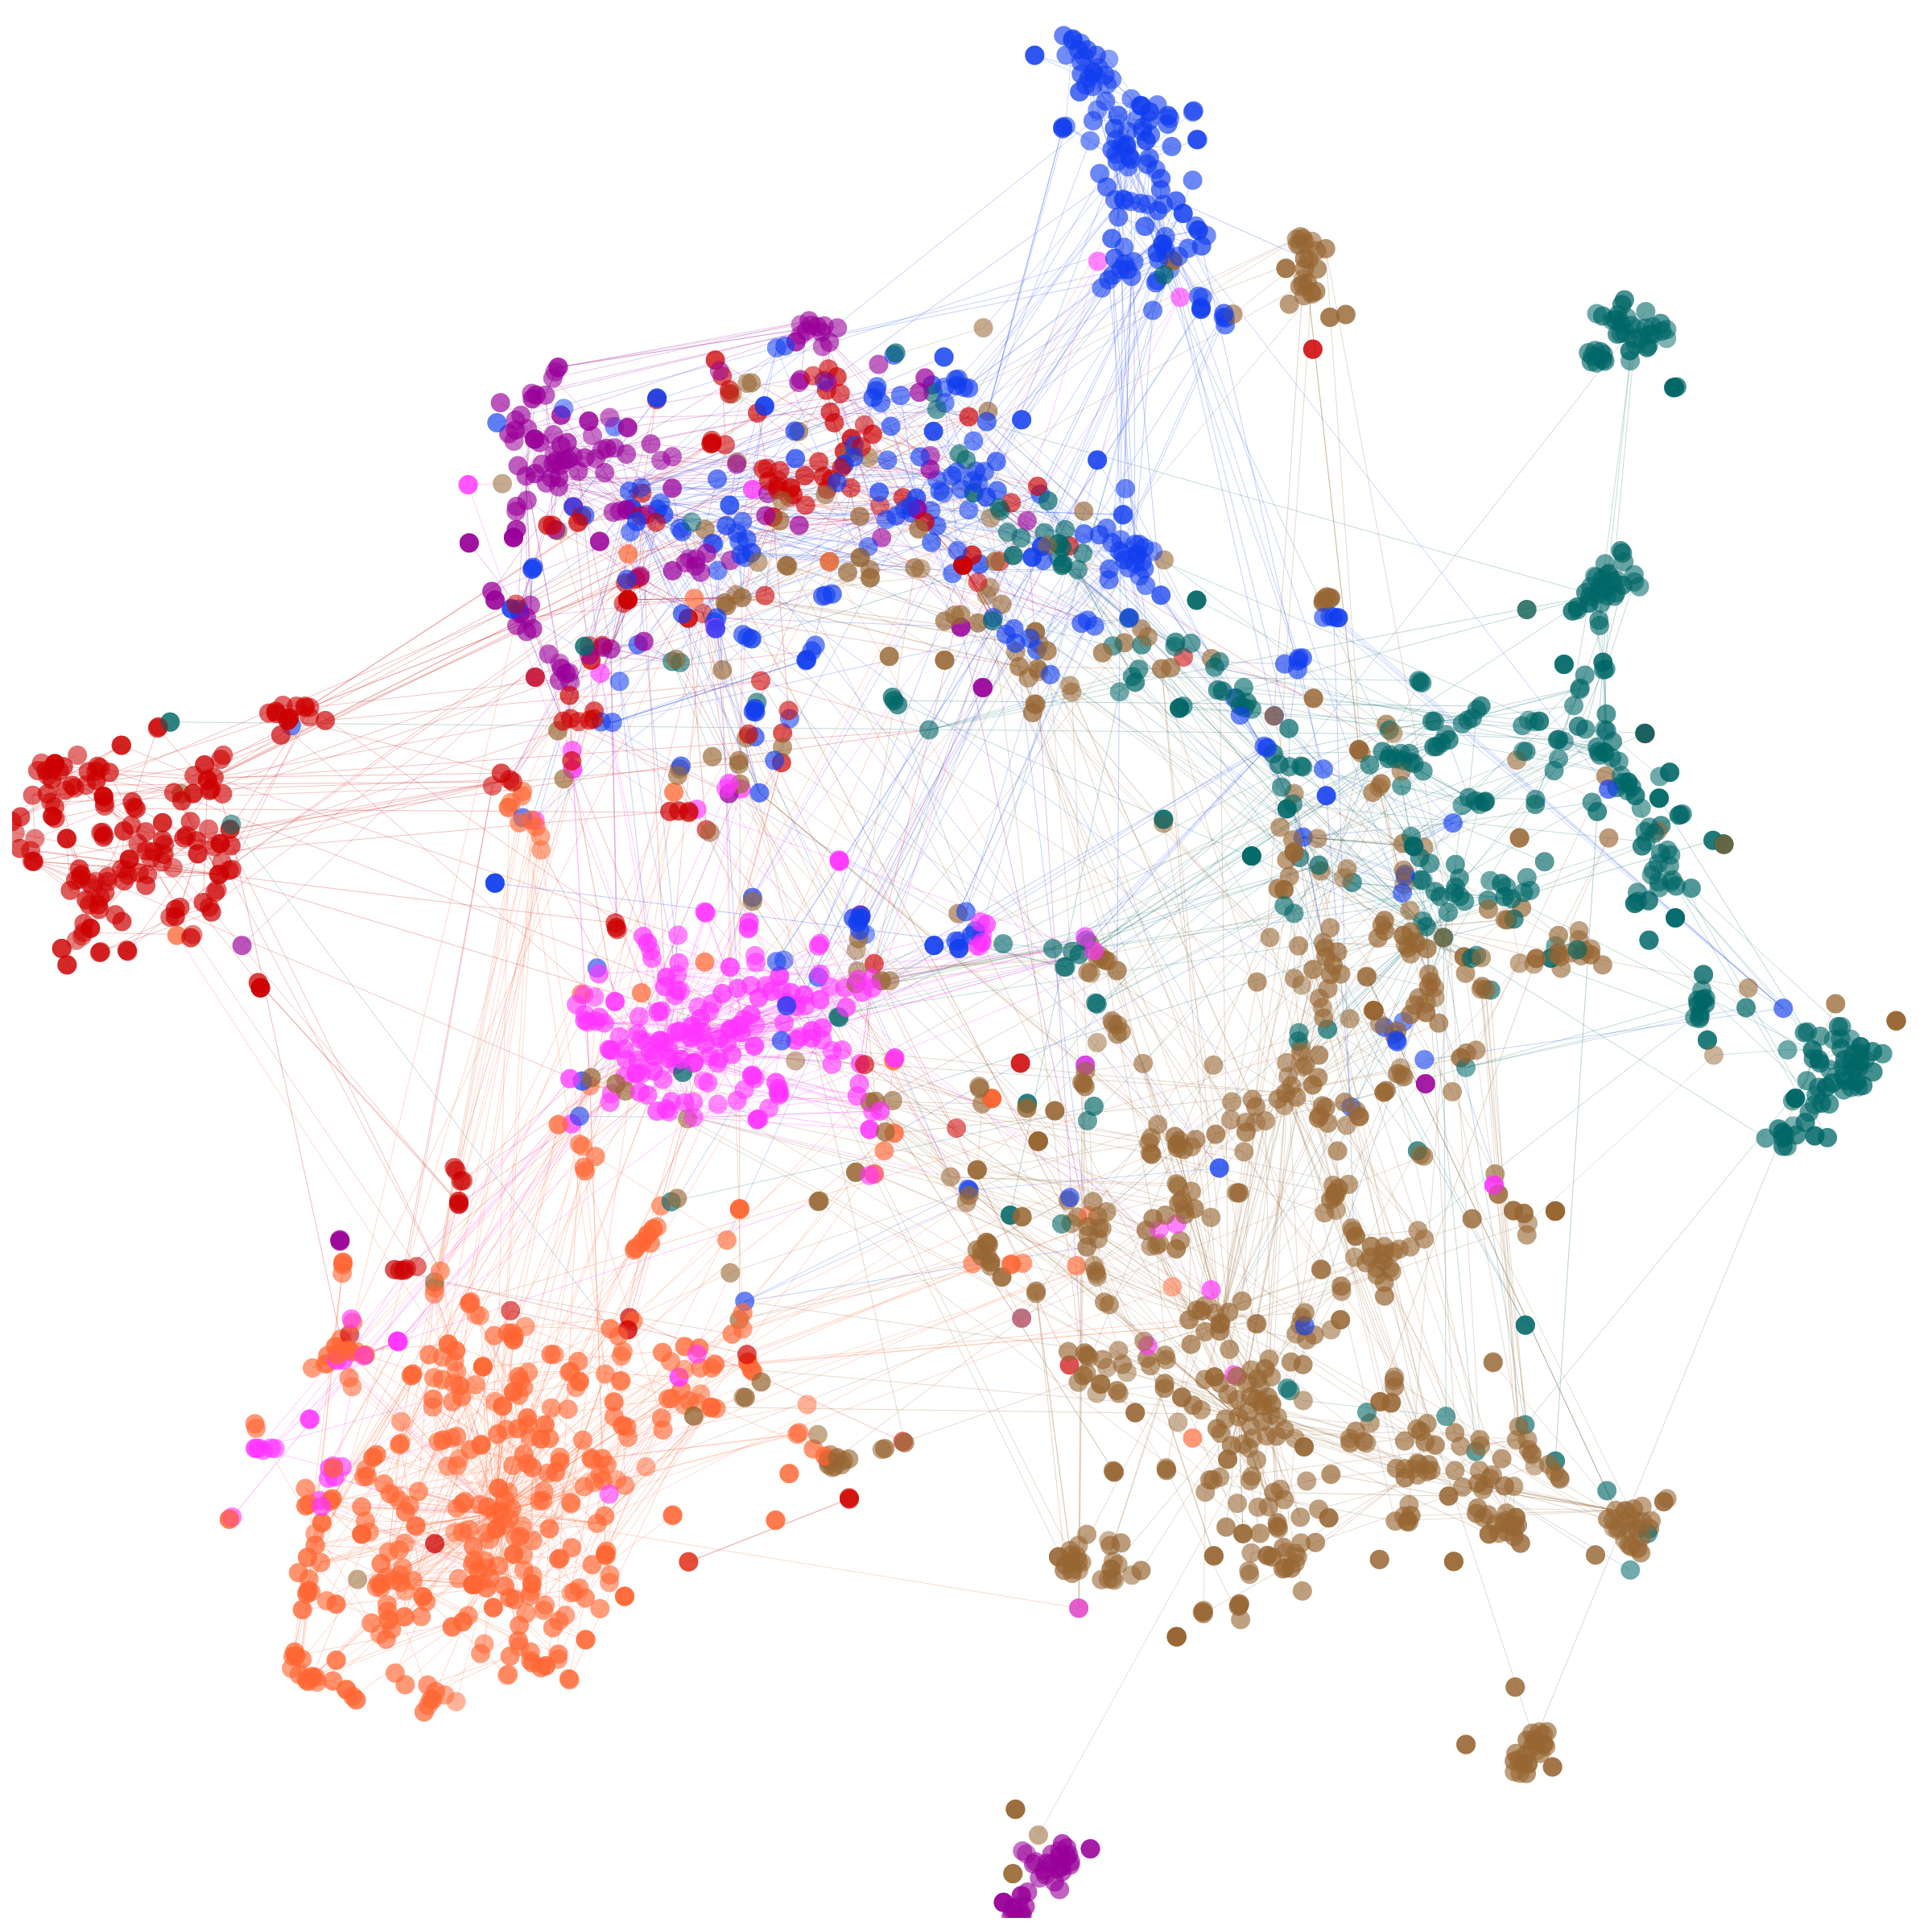
\includegraphics[width=0.15\linewidth]{figure/RHGNN_cora_visualization.png}
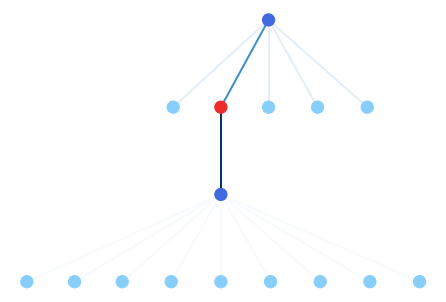
\includegraphics[width=0.15\linewidth]{figure/cora_att.png}
}
\subfigure[WebKB $\delta = 1$]{
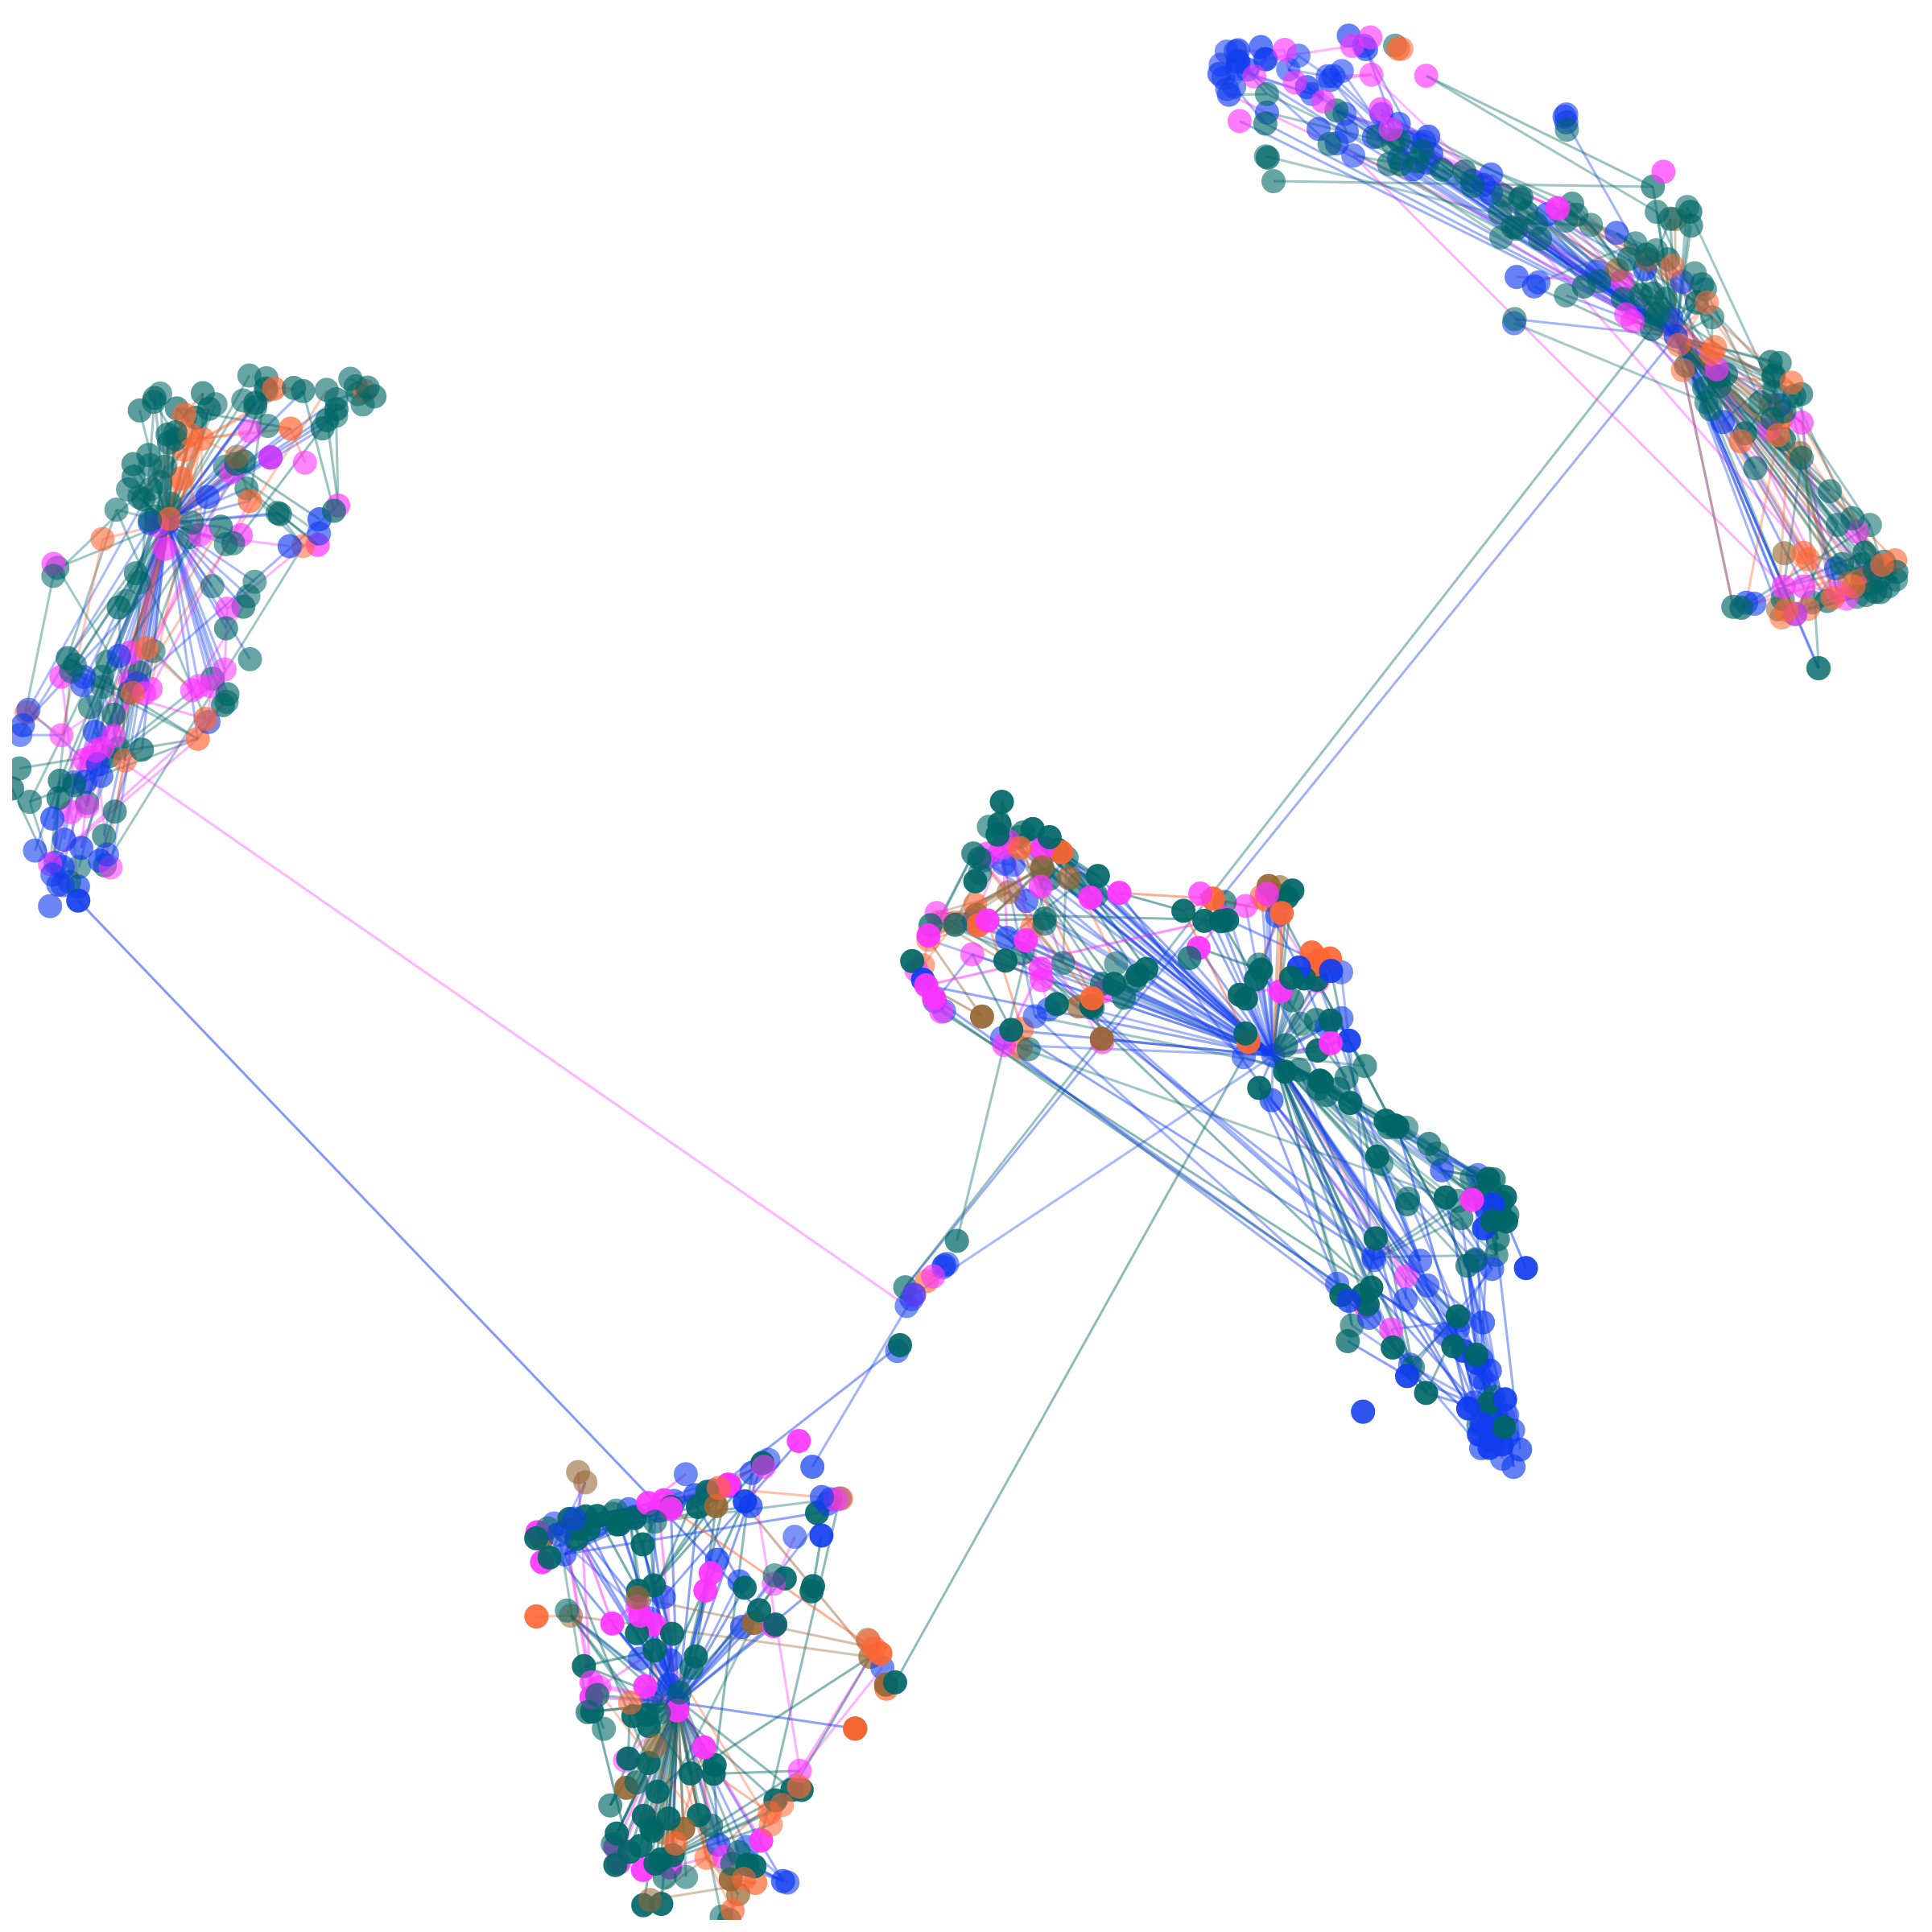
\includegraphics[width=0.15\linewidth]{figure/RHGNN_webkb_visualization.png}
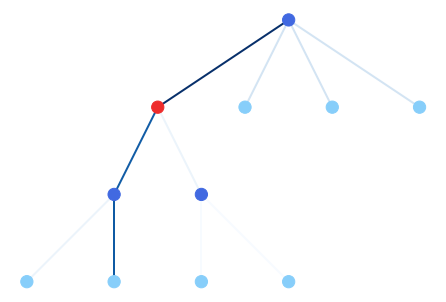
\includegraphics[width=0.15\linewidth]{figure/webkb_att.png}
}
\centering
\caption{Embeddings (left) and attention weights (right) visualization of RAHGNN on datasets with different $\delta$.}
\label{visualization2}
\end{figure*}

\subsection{Reinforcement Learning Analysis}
\subsubsection{RL Process Analysis.}
We plot the training process of RAHGNN to verify the effectiveness of the reinforcement learning mechanism in Figure \ref{RL_loss}, where each plot shows the trend of ROC-AUC or Accuracy for the HGNN Agent during the whole training process. The shadowed area flags min or max train metrics in a 5-fold cross validation run, and the solid line indicates the mean value. On the downstream tasks of each dataset, RAHGNN converges within a few hundred epochs.

\subsubsection{Curvature Learning analysis.}
Figure~\ref{LP-C} shows the curvature updating process of RL in different datasets and tasks. 
The blue line is the curvature of the first hyperbolic graph neural layer in HGNN, and the orange line is the curvature of the second hyperbolic graph neural layer. In most cases, when the model ends training, the curvatures also show a trend of converging to fixed values around.  We observe that the optimal curvature in the first layer is less than the one in the second layer in Pubmed and Cora with high $\delta$-hyperbolicity, while it is the opposite in WebKB and PPI with less $\delta$-hyperbolicity. 
Moreover, it is obvious that the curvatures of two HGNN layers present a close relationship with competition and cooperation: in several adjacent epochs, the curvatures of two HGNN layers often choose opposite actions simultaneously or remain unchanged at the same time; but on the scale of the entire training process, the overall trend of two layers is the same.


\begin{table}[htb]
\caption{ROC of RAHGNN with Möbius operations (RAHGNN-M) and Einstein midpoint (RAHGNN-E) for link prediction}
\begin{tabular}{lccccc}
\toprule
\textbf{Method} & \textbf{Citeseer} & \textbf{Cora} & \textbf{Pubmed} & \textbf{PPI} & \textbf{WebKB} \\ 
\midrule
RAHGNN-M         & 95.82          &  \textbf{93.22} & 93.96          & \textbf{91.60} & 93.55          \\
RAHGNN-E         & \textbf{96.94} &  91.52          & \textbf{94.87} & 91.30          & \textbf{94.32} \\ 
\bottomrule
\end{tabular}
\label{ablation}
\end{table}

\subsection{Model Analysis}
There are two main ways to compute the feature aggregation in hyperbolic neural networks: Möbius operations~\cite{HNN:GaneaBH18,HGCN_ChamiYRL19} and Einstein midpoint~\cite{HAtt}. 
% The different between Möbius operations and Einstein midpoint is: 
The Möbius operations perform the aggregation operation by using exponential mapping to project embeddings into the tangent space, and then projecting back to the hyperbolic space by logarithmic mapping. 
The Einstein midpoint is computed directly in hyperbolic space, equivalent to the weighted sum of Euclidean space. 
We further analyze the effect of two hyperbolic aggregation operations of graph in our proposed framework, namely RAHGNN+M (RAHGNN with Möbius operations) and RAHGNN+E (RAHGNN with Einstein Midpoint). 
We observe different aggregation performance of graph via these two computation operations in hyperbolic space with different curvature.
As shown in Table~\ref{ablation}, the performance of RAHGNN+E is similar to RAHGNN+M, but RAHGNN+E has a slight advantage in our experiments. 



\subsection{Visualization}
For a more intuitive comparison and to further show the effectiveness of our proposed model, we show the visualization of Cora in Figure~\ref{visualization1}. 
We visualize the embeddings of nodes in the test set by t-SNE~\cite{van2008visualizing}. The nodes are labeled with 7 different colors. 
As shown in Figure~\ref{visualization1}, HGCN and RAHGNN cluster nodes in a better separation way compared with the results of GCN and GAT. 
In contrast to HGCN, RAHGNN indicates higher intra-class similarity and the clearer distinct boundaries among different classes. 

Figure \ref{visualization2} illustrates the corresponding embeddings and attention weights in and the 2-hop neighborhood of a center node (red) for three datasets with various $\delta$. 
We visualize the attention weights for the red nodes. 
The hierarchy of the nodes are visualized by the darkness of the color. 
The intensity of edges between the neighbours denotes the attention weights of nodes. 
We observe that the center nodes are more concerned about their (grand)parents in datasets with lower $\delta$. 
In contrast to Citeseer, the aggregations with attention in Cora and WebKB pay more attention to the high hierarchy of nodes. 
Such attention is vital to good performance in datasets with different hierarchies.